\documentclass{article}
\usepackage[utf8]{inputenc}
\usepackage[spanish]{babel}
\usepackage{listings}
\usepackage{graphicx}
\graphicspath{ {images/} }
\usepackage{cite}

\begin{document}

\begin{titlepage}
    \begin{center}
        \vspace*{1cm}
            
        \Huge
        \textbf{Analisis Parcial II - Informatica II.}
            
        \vspace{0.5cm}
        \LARGE
            
        \vspace{1.5cm}
            
        \textbf{Luis Miguel Gil Rodriguez.}
        \\
        \textbf{Maverick Sossa Tobon.}
        \vfill
        \vspace{0.8cm}
            
        \Large
        Despartamento de Ingeniería Electrónica y Telecomunicaciones\\
        Universidad de Antioquia\\
        Medellín\\
        Septiembre de 2021
            
    \end{center}
\end{titlepage}
\tableofcontents
\newpage
\section{Sección introductoria} \label{intro}
En este documento, podremos encontrar las ideas para abordar el parcial numero dos del curso Informatica II. Encontraremos en el detalles tales como el lgoritmo de redimensionamiento de imagenes para luego se mostrados en una martriz de LEDs de un tamaño ce 16 por 16 LEDs.

\section{Analisis del Problema} \label{Analisis}
Desde un principio se tuvo en mente que nuestro algoritmo debe estar en capacidad de redimensionar imágenes que sean tanto mas chiquitas como mas grandes que nuestra matriz de LEDs de 16 X 16.
\\
\\
En lo que respecta al procesamiento de la imagen, se deduce que puede haber 5 casos:
\begin{enumerate}
    \item La imagen sea de 16 X 16 (Caso ideal).
    \item El ancho sea mayor que 16 pero el alto menor que 16.
    \item El ancho sea menor que 16 pero el alto mayor que 16.
    \item EL ancho y el ato mayores que 16.
    \item El ancho y el alto menores que 16.
\end{enumerate}
En los casos 2 y 5 pueden haber 4 subcasos:
\begin{enumerate}
    \item La división entre el ancho y 16 sea entero.
    \item La división entre el ancho y 16 sea decimal.
    \item La división entre el alto y 16 sea entero.
    \item La división entre el alto y 16 sea decimal.
\end{enumerate}
Seguido de eso, surgió una primera idea para el algoritmo de redimensionamiento, el cual seria en dividir la imagen en 16 X 16 cuadriculas para un total de 256 subregiones, con el objetivo de recorrer cada una de ellas y sacar un promedio de la intensidad de rojo, verde y azul de cada píxel que abarca la subregión, en la matriz de LEDs se mostraría el promedio de cada uno de los colores.
\\
\\
Surgió un segundo algoritmo, el cual involucra dividir la imagen como se describió en el anterior algoritmo, seleccionar los datos de la mitad y realizar un promedio entre ellos. La intensidad de cada color de dicho promedio es el que se va mostrar en la matriz de LEDs.
\\
\\
El tercer algoritmo que surgió fue con respecto a la moda (el dato, en este caso intensidad de color que más se repite en la subregión), la moda de cada subregión será la que se va a mostrar en la matriz de LEDs.
\\
\\
Se debe de tener en cuenta que al dividir la imagen en 256 cuadriculas, el alto y el ancho de cada una de ellas (subregión) sea un numero decimal, por ende, se debe tomar la parte entera de dicho número y la suma de los residuos será el tamaño del ancho o alto de la última subregión.
\\
\\
La metodología de los algoritmos anteriormente descritos tiene sentido cuando ancho y alto de la imagen a aplicarle el algoritmo es mayor a 16, por ende también se pensó como proceder cuando uno de estos sea menor a 16, en este caso, se debe dividir entre 16 el ancho o el alto de la imagen, y dicho número representará la cantidad de veces que se repetirá el dato en la matriz de LEDs.
\\
\\
Se planea desarrollar y evaluar cada uno de los algoritmos aquí descritos para mirar cuales son sus fortalezas y debilidades, y como podemos emplear cada uno de ellos en un escenario en específico.
\\
\\
Luego de que el programa de QT aplique el algoritmo de redimensionamiento sobre la imagen, el programa debe estar en la capacidad de generar un archivo de texto que dentro del contenga tres matrices, cada matriz tendrá 256 elementos, los cuales representaran la intensidad de cada uno de los colores RGB. La información de ese archivo de texto debe ser tal como:
\\
\\
\begin{lstlisting}[language=C++, label=codigo_ejemplo]
RedMatrix [16][16] = {...};
GreenMatrix [16][16] = {...};
BlueMatrix [16][16] = {...};
\end{lstlisting}
O se esta pensando en generar una matrices unidimensionales:
\\
\\
\begin{lstlisting}[language=C++, label=codigo_ejemplo2]
RedMatrix [256] = {...};
GreenMatrix [256] = {...};
BlueMatrix [256] = {...};
\end{lstlisting}
Las cuales van a ser copiadas directamente al código de Tinkercad para que se muestre en la matriz de LEDs.

\section{Algoritmo} \label{algoritmo}
En el planteamiento del algoritmo solución se defininen, de forma general, las subtareas y datos que unidos y ordenados permiten obtener el cometido: un programa de redimensionamiento de imagenes. Entonces, para tener una idea aproximada del funcionamiento de tal programa, se hace necesario describir ciertos subprocesos. 

\subsection{Inicialización} \label{Inicializacion}
En el intanciamiento de un objeto quien se enccarga de inicializar ciertos datos es el contructor. 
El constructor sobrecargado recibirá: 
\begin{enumerate}
  \item Tamaño del redimensionamiento.
  
  En primera instancia corresponde a las dimensiones de la matriz de leds RGB de 16x16 que se planea usar para la solución del problema.
  Esto para adaptarlo a otra posible matriz de leds de dimensiones distintas. 
  \item Nombre archivo .txt
  
  Corresponde al único dato que debe ingresar el usuario: el nombre del archivo donde se almacenará el segmento de código correspondiente a las matrices, las cuales contendrán los datos de la imágen ya redimensionada. 
  Es una ruta relativa, en usuario debe conocer la ubicación de tal archivo .txt.
  
\end{enumerate}
\subsection{Atributos} \label{Atributos} 
En la creación de la clase, los atributos definen características importantes del objeto y almacenan datos necesarios para la ejecución de ciertos métodos. 

\begin{enumerate}
  \item Matrices bidimensionales de cada color
  
  Tres corresponden a los datos de la imagen redimensionada. 
  Una para rojo, otra para verde y otra para azul. Se obtendrá con la ejecución de métodos, y despues, con otro método, se guardará en un archivo .txt.
  
  \item Ancho y largo de la redimensión
  
  Fueron inicializados en el constructor. Se usarán constantemente, pues son las dimensiones a la cual se quiere llegar.
  
  \item Objeto QImagen
  
  Se obtiene a partir del dato ingresado por el usuario: la ruta a la imagen a redimensionar. Con él se tendrá acceso a todos los datos de la imagen, los cuales serán usados en el proceso de redimensionamiento bajo un algoritmo implementado que cumple 
  
\end{enumerate}

\section{Circuito.} \label{circuito}
Para la implementación del circuito en la plataforma Tinkercad, primeramente se comenzaron a realizar ensayos con una tira de 16 Neopixeles, la cual se conecta de la siguiente manera:
\begin{enumerate}
  \item La primera fila se conecta al puerto 2 del Arduino.
  \item Se le suministra potencia de 5 Voltios a la tira de Neopixel procedentes del Arduino.
  \item Se conecta el polo a tierra procedente del Arduino a la tira del Neopixel.
\end{enumerate}
\begin{figure}[h]
  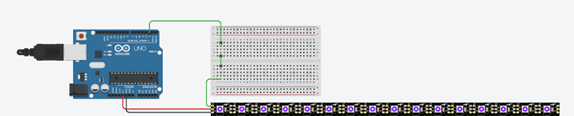
\includegraphics[width=10cm]{figura_1.png}
  \centering
  \caption{Prender fila numero uno de la matriz.}
  \label{fig:fila_uno}
\end{figure}
Se comenzó la etapa de pruebas con la tira de Neopixel, ejemplo de algunas pruebas que se realizaron:
\begin{enumerate}
    \item Cómo prender un Neopixel en específico.
    \item Cómo mostrar un patrón en una tira (ejemplo: Solo prender las posiciones impares, solo prender las posiciones pares).
    \item Cómo prender todos los leds e a la vez.
\end{enumerate}
Una vez superada esta etapa de prueba se agregaron las 15 filas restantes, para obtener una especie de matriz de 16 X 16, en primer lugar se realiza la conexión desde la fila uno hasta la fila cinco de la siguiente manera:
\begin{enumerate}
    \item Se conecta entrada de la fila N con la entrada de la fila N+1.
    \item Se conecta la potencia de la fila N con la potencia de la fila N+1.
    \item Se conecta la tierra de la fila N con la tierra de la fila N+1.
\end{enumerate}
Al intentar interactuar con la matriz, por ejemplo prender una Neopixel en específico se evidencio que tenía un comportamiento de prender por columnas, conducta para nada esperada.\\
\begin{figure}[h]
  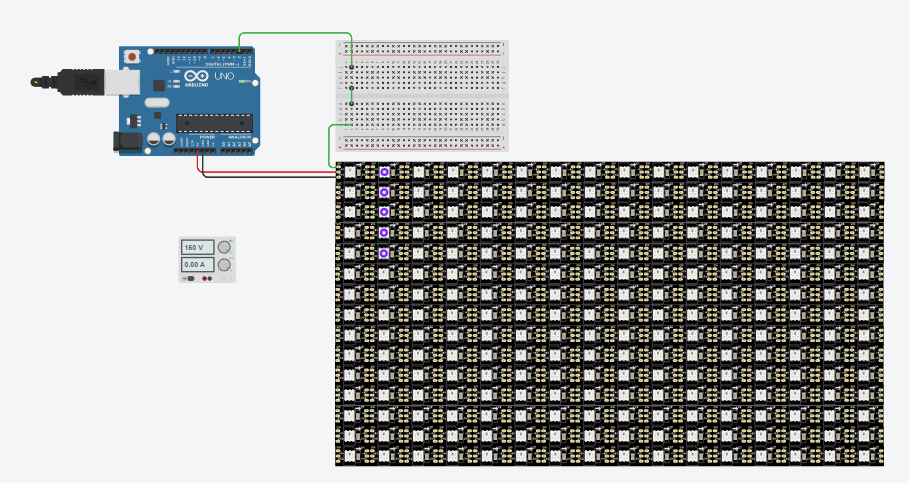
\includegraphics[width=10cm]{figura_2.png}
  \centering
  \caption{Comportamiento no esperado.}
  \label{fig:por_columnas}
\end{figure}
Al evidenciar este comportamiento, de inmediato se repiensa la manera de como realizar satisfactoriamente la conexión. Hasta que se llego hasta la siguiente idea:
\begin{enumerate}
    \item Se conecta salida de la fila N con la entrada de la fila N+1.
    \item Se conecta la potencia de la fila N con la potencia de la fila N+1.
    \item Se conecta la tierra de la fila N con la tierra de la fila N+1.
\end{enumerate}
Luego de haber realizado dicha conexión, se comenzó una nueva etapa de pruebas con el mismo, se intento prender todas las filas conectas, un Neopixel en específico y por último un patrón sencillo, como prender solo las posiciones impares, la diagonal principal de la matriz entre otras pruebas.

\centering
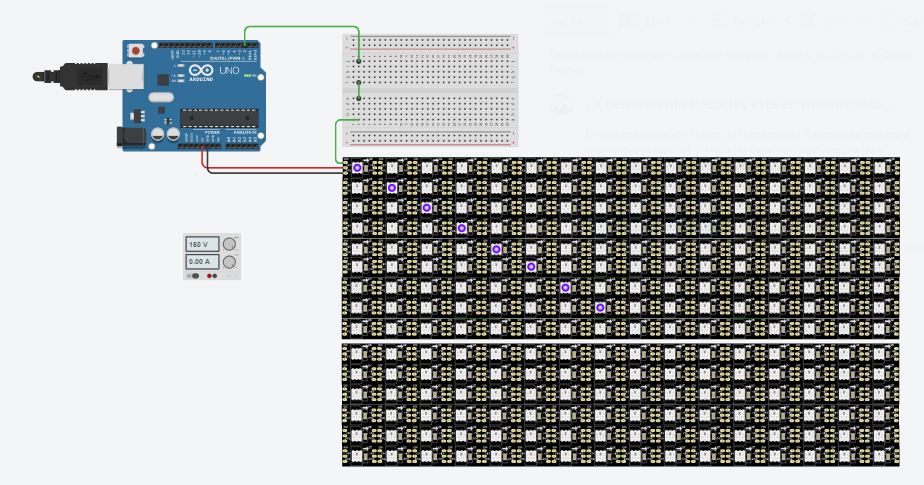
\includegraphics[width=8cm]{figura_3.png}
  
A continuacion se mostrara el circuito desarrollado, cabe mencionar, que el aspecto que aqui se muestra no sera el definiticvo, pues se reorganizaran las tiras de Neopixel de una manera mas estetica.

\centering
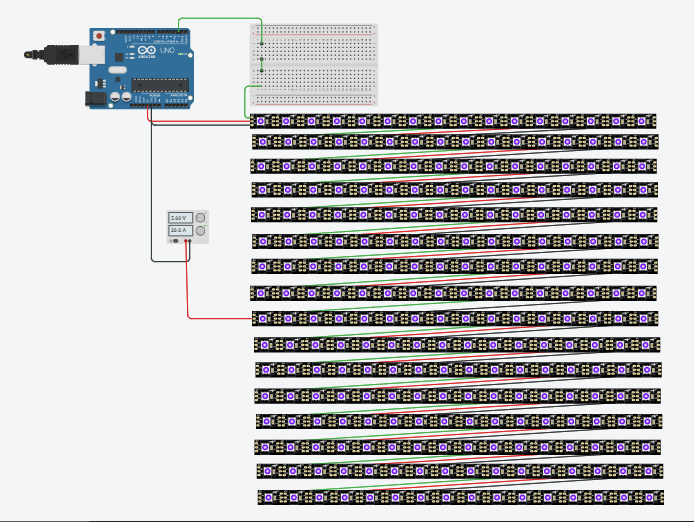
\includegraphics[width=8cm]{figura_4.png}

\begin{enumerate}
    \item Los cables de color verde se encargan de llevar los datos a la matriz de LEDs
    \item Los cables de color Negro representan el Polo a Tierra.
    \item Los cables de color Rojo representan la potencia (5.0 V).
    \item Se conecta un suministro de energia, el cual alimentara la matriz de LEDs, es decir suministrara potencia a partir de la fila 9 de nuestra matriz. Este mismo alimentará con 5.0 Voltios a la matriz de LEDs.
\end{enumerate}
\bibliographystyle{IEEEtran}
\bibliography{references}
\end{document}